\documentclass{article}
\usepackage[utf8x]{inputenc}
\usepackage{times}
\usepackage[intlimits,sumlimits]{amsmath}
\usepackage{amssymb}
\usepackage{graphicx}
\usepackage{hyperref}
% listings begin
\usepackage{color}
\usepackage{xcolor}
\usepackage{listings}
\usepackage{caption}
\DeclareCaptionFont{white}{\color{white}}
\DeclareCaptionFormat{listing}{\colorbox{gray}{\parbox{\textwidth}{#1#2#3}}}
\captionsetup[lstlisting]{format=listing,labelfont=white,textfont=white}
% listings end
%opening
\author{Milán Unicsovics}
\title{Project Laboratory 1}
\date{\today}

% Prevent too long lines
\sloppy
\begin{document}
%%%%%%%%%%%%%%%%%%%Titlepage%%%%%%%%%%%%%%%%%%%%%%
\begin{titlepage}

\begin{figure}[htp]
\centering
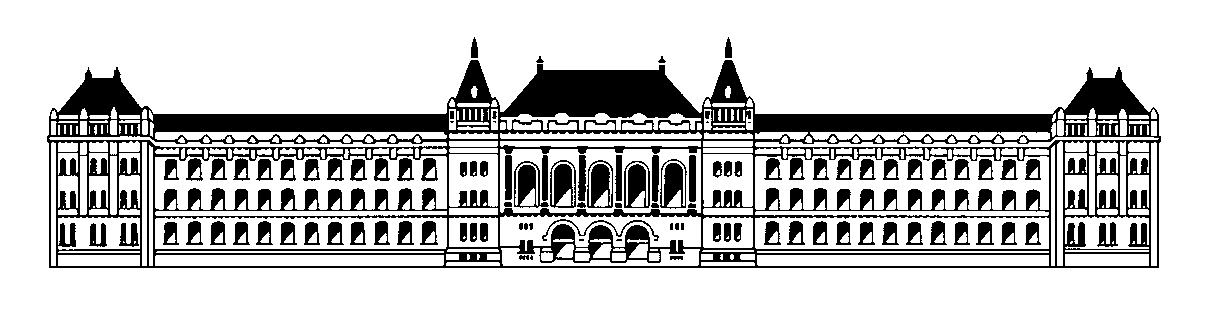
\includegraphics[scale=0.3]{img/bme.png}
\begin{center}
Budapest University of Technology and Economics\\
Department of Measurement and Information Systems
\end{center}
\end{figure}

\vspace{3cm}
\begin{center}
\textsc{\LARGE \textbf{Test generation based on state machine models}}
\vspace{0.5cm}\\
Project Laboratory 1 final report\\
2013/14. I. semester

\vspace{3cm}
\textsc{\large \textbf{Milán György Unicsovics (M9GNTV)}}
\vspace{0.5cm}\\
I. year, computer engineering student\\
MSc Specialization in Dependable System Design

\vspace*{\fill}

Consultant:\\
Dr. Zoltán Micskei assistant professor, MIT\\[0.3cm]

\end{center}

\end{titlepage}
%
\tableofcontents
\newpage
%%%%%%%%%%%%%%%%%%%Text%%%%%%%%%%%%%%%%%%%%%%

\section{Introduction}
\label{sec:intro}

The main goal of software testing is fault detection, where we compare the software's intended and actual behaviour to make sure there are not any difference between those, regarding the requirements.

These methods are usually very time and resource consuming activities. The process is often undocumented, unrepeatable and unstructured, that's why creating tests limited by the ingenuity of the single developer. Furthermore the traditional test cases are static and hard to update, but the software under test is dynamically evolving. One other problem of the handcrafted test is, that they suffer from "pesticide paradox". The test are getting less effective during the testing process, because the tester writes them with the same method for mostly solved problems.

Model-based testing substitutes the traditional ad-hoc software testing methods which relies on behaviour models that describe the intended behaviour of the system and its environment. From the models set of test cases are generated automatically and then executed on the tested software.

My research aims to prepare to create a new automated testing framework for software based on state machine models. Before that related works and similar solutions have to be examined. The result of the research later can be used to design and develop a software which fills the need of a fully automated model based testing framework.

% section intro (end)

\section{Model-based testing}
\label{sec:mbt}

The idea of model-based testing originates from the 70's, and now it has an extensive literature, terminology and a commonly accepted taxonomy \cite{taxonomy}. This section introduces the concept of this variant of software testing through a concrete process (Figure~\ref{fig:mbtprocess}).

\begin{figure}[htp]
\centering
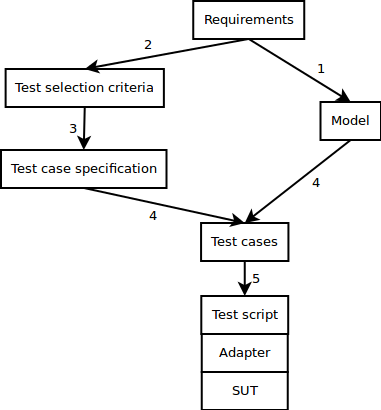
\includegraphics[scale=0.6]{img/mbt_process.png}
\caption{Model-based testing process}
\label{fig:mbtprocess}
\end{figure}

\begin{enumerate}
    \item From informal requirements or created specifications a model can be built. The model is an abstract representation of the \textit{system under test (SUT)}. It uses encapsulation to information reduction, because it has to be more simple, than the original system to achieve an easier modifying, maintaining \cite{mbttestcasegeneration}. During a model-based software development it can be used for many other tasks too, as the model serves analysing, synthesising and documenting the SUT as well.
     \item Test selection criteria decide how the test cases are chosen, which point of view is important by testing. Further details are at the subsection~\ref{sub:taxonomy}.
     \item Criteria are transformed into test case specifications. These test case specifications are the formalised versions of the critera.
     \item After creating the model and the test case specifications set of test cases is generated from the model regarding all the specifications. One of the biggest challenges is to create the \textit{test cases}. A simple test case consists of a pair of input parameters and expected outputs. Finite set of test cases forms a \textit{test suite}. The difficulty comes from the need to satisfy the test case specifications and create a minimised set of test cases.
     \item A successfully generated test suite can be executed on the SUT. For the execution a \textit{test script} can be used, which executes the test cases.
     
     The generated test cases are strongly linked to the abstract test model, therefore an \textit{adaptor} component is needed, which is often part of the test script. The adaptor adapts the test inputs to the SUT. For example if the input of a method is an XML document containing an integer value, the adaptor has to transform the test case's test inputs to XML.
     
     The test script also contains usually a \textit{test oracle}, that checks the test output difference from the expected output.
\end{enumerate}

\subsection{Taxonomy}
\label{sub:taxonomy}

Utting, Pretschner and Legeard investigated the currently available MBT solutions and defined (Figure~\ref{fig:mbttaxonomy}) a taxonomy which concentrates to three major properties of model-based testing. The three dimensions of their taxonomy are the modelling specification, test generation and test execution.

\begin{figure}[htp]
\centering
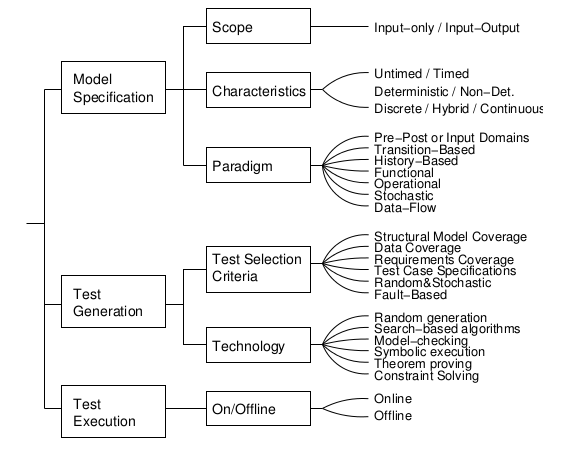
\includegraphics[scale=0.5]{img/mbt_taxonomy.png}
\caption{Model-based testing taxonomy \cite{taxonomy}}
\label{fig:mbttaxonomy}
\end{figure}

\begin{description}
	\item[Model scope] The scope of the modelling is a binary decision. The model either specify \textit{just the test input} or \textit{the input-output pairs} for the SUT. The first case is less useful, because the test script can not check the SUT's output and that's why it is impossible to create an oracle that way.
	
	\item[Model characteristics] The SUT assigns the main characteristics of the model. It depends on the SUT's timing properties (\textit{timed} / \textit{untimed}), determinism (\textit{deterministic} / \textit{non-deterministic}) and dynamics (\textit{discrete} / \textit{continuous} / \textit{hybrid}).
	
	\item[Model paradigm] The third dimension is the paradigm that is used to describe the model. \textit{State-based notation} means, that set of variables defines the model, which represents the internal state of the system. By \textit{transition-based notation} the model focuses on the transition between the state of the system. Finite state machines are examples for this paradigm. \textit{History-based notations} model the allowable traces of its behaviour over time. By \textit{functional notation} collection of mathematical functions model the system. \textit{Operational notations} describe the model as a set of executable processes running parallel. \textit{Stochastic notations} describe the model by a probabilistic model, as it is rather suitable to model the environment than the SUT itself. The last paradigm is the \textit{data-flow notation}, where the main concept is the concentration to the data, rather than the control flow.
	
	\item[Test selection criteria] Test selection criteria control the test case generation. \textit{Structural model coverage criteria} aim to cover a part of the model, for example nodes and arcs of the transition-based model. The basic idea of \textit{data coverage criteria} is to split the data space to equivalence classes and choose values from them. \textit{Requirements based coverage criteria} are linked to the informal requirements of the SUT and it applies the coverage to the requirements. \textit{Ad-hoc test case specifications} guides by the test case specifications. \textit{Random and Stochastic criteria} are useful rather to model the environment and applicable to use with a stochastic model. \textit{Fault-based criteria} can be very efficient, because it concentrates to error finding in the SUT.
	
	\item[Test generation technology] One of the most important thing that defines the test case generation is the chosen technology. The easiest one to implement is the \textit{random generation}, more difficult are the \textit{search-based algorithms} where graph algorithms and other search algorithms are used to perform a walk on the model. \textit{Model checking} can also be used for test case generation, where the model checker searches for a counter-example, which becomes a test case. \textit{Symbolic execution} means analysing the software to determine what inputs cause each part of a program to execute. This method guided by test case specification to reach a goal, and test inputs become inputs which produce different outputs. \textit{Deductive theorem proving} is similar to model checking, but the model checker is replaced with a theorem prover. \textit{Constraint solving} is useful for selecting data values from complex data domains.
	
	\item[Test execution] The tests can run either \textit{online} or \textit{offline} on the SUT. During an online test, the test generator can respond to the SUT's actual output for example with an different test case sequence. By an offline test generation test cases are generated strictly before the execution.
	
	The testing can be started by an automatic execution or manually, that triggers the user directly.
\end{description}

% subsection taxonomy (end)

% section mbt (end)

\section{Tools review}
\label{sec:toolsreview}

Model-based testing is a mature idea, and it has an extensive literature. Nevertheless the number of the available tools is less than we can expect that. To really take advantage of model-based testing, reliable tools and automation support are required. A usable model-based testing tool has to help in the whole testing process. That means creating and verifying the model, generating test cases, constructing test scripts, adaptors and oracles. Utting, Pretschner and Legeard \cite{taxonomy} defined MBT as testing that relies on models specifying the intended behaviour of the SUT. In reality that would mean restricting MBT to black-box testing, where we can only generate abstract test cases from the behaviour model. That's why Shafique and Labiche defined MBT as a support of software testing activities from a model of the SUT behaviour. We follow this point of view in this paper.

Shafique and Labiche \cite{toolsreview} collected the available tools that rely on state-based models and created a systematic review considering the previously and newly defined criteria.

\begin{description}
	\item[Model-flow criteria] This criterion details the state-based coverage options and applicable to state-based models, which belong to transition-based models. The coverage options can be state, transition, transition-pair, sneak path, all-paths and scenario criteria. The first five are well-known, scenario criteria means, that the test should follow user defined test sequence to pass.
	\item[Script-flow criteria] This criterion refers to interface (function), statement, decision/branch, condition, modified-condition/decision and atomic-condition. They can extend the finite state machine's mechanism. Interfaces refer to the functions which are called on the SUT, the others can serve as guards on transitions.
	\item[Data criteria] This criterion refers to the selection of input values when creating concrete test cases from abstract test cases. The options are one-value, all-values, boundary-values and pair-wise values. By one-value only one concrete test case will be generated for an abstract test case, by all-value all concrete test case will be generated for an abstract test case. Boundary-value means selecting values from a specific range.
	\item[Requirement criteria] It is a binary decision whether a tool supports checking of requirement's satisfaction or not. Requirements are linked to a specific part of the model (e.g.: transition, state).
	\item[Scaffolding criteria] Scaffolding means generating part of a required code. Fully support refers to scaffolding out all needed part of the process, partially support means only a few of them.
\end{description}

\subsection{GraphWalker}
\label{sub:graphwalker}

The first investigated tool was GraphWalker \cite{graphwalker}, which can create online and offline tests from finite state machines, extended finite state machines or from both of them. The framework is written in Java, the related tools belong to Java world as well. Maven is used to run the tests, TestNG to describe the test cases.

The input model has to be in GraphML format, which is an easy-to-use, highly extendable XML extension for describing graphs. The creators of this software think that UML is too complex, and its functionality is not necessary by software testing, that's why they chose this format. Recommended tool to create GraphML is yED, which is a graphical graph editing software.

After designing the model, test stubs, adaptors and oracles will be generated. The test stub has to be filled with the linking logic with the SUT. While running the tests GraphWalker can use different methods to walk on the state space. For example A* search, shortest path, random path, all permutation. The tests will stop when a certain stop criterion has been satisfied. The stop criteria are state coverage, transition coverage, requirement coverage and time limit.

% subsection graphwalker (end)

\subsection{PyModel}
\label{sub:pymodel}

PyModel \cite{pymodelarticle}\cite{pymodel} is an open-source MBT testing framework written in Python. It consists three main tools:

\begin{description}
	\item[pma - PyModel Analyzer] It validates the model and creates FSM from it.
    \item[pmg - PyModel Graphics] It generates graphical representation of the FSM.
    \item[pmt - PyModel Tester] It creates online and offline test cases and executes them.
\end{description}

PyModel's test input has to be created by code. The methods will be the transitions in the FSM, states are the defined attributes. It is possible to combine different models in a test. Scenarios supported as well, so user can guide the tests with a given test case sequence. There are two test coverage criteria, state-based and transition-based coverage.

% subsection pymodel (end)

\subsection{Conclusion}
\label{sub:conclusion}

After examining the available tools the result is the following:

\begin{itemize}
	\item The tools implement different coverage criteria, but mostly just the easiest ones (state-based and transition based version of structural model coverage criteria). More difficult criteria are avoided, for example data coverage, requirement-based and fault-based criteria and transition pairs coverage from structural coverage criteria.
	\item Script-flow criteria are rarely used techniques. Only a few tools support guards on transitions or use scripts for example to give control information of the SUT.
	\item Scaffolding solutions of the tools are incomplete. Fully automatic generation of test adaptors, oracles are seldom supported.
	\item Regression tests are not supported.
\end{itemize}

% subsection conclusion (end)

% section toolsreview (end)

\section{Connection with graph theory}
\label{sec:mbtgraphtheory}

In the last few decades there has been an exhausting research in the field of using graph theory at model-based testing. These techniques belong to search-based test generation algorithms.

One of the most used algorithms refers to the \textit{Chinese Postman Problem} \cite{graphtheorymbt}. Given that it is impossible to cross each edge once in an undirected graph during a graph walk, in other words it does not have an Eulerian tour. What is the minimal amount of re-crossing we need to create a walk that uses each edge? The solution is to duplicate the shortest edges between the vertices having odd degree. This process is called "Eulerizing" the graph. In model-based testing one can use this idea, by creating a transition-based model, which can be represented as a graph. The vertices are the states of the SUT and the edges are the callable methods. A generated Eulerian tour gives a full transition-based structural model coverage.

The \textit{New York Street Sweeper Problem} is a variant of the previous graph theory problem. It applies to directed graphs, and arcs need to duplicate to reach, that each nodes have out-degree minus in-degree equal zero.

The previous algorithms give full transition-based coverage, but not pair-wise coverage. The following algorithm named \textit{de Bruijn sequences} creates every combination of the methods. First create a dual graph of the original graph, then eulerize the dual graph (by duplicating arcs to balance node polarities). Create an Eulerian tour, noting the names of the passed nodes.

Dill, Ho, Horowitz and Yang constructed worked on the \textit{limited sub-tour problem} where the test case sequences can not be longer, than a specified upper limit. There is no optimal solution for that problem, but there are some heuristics. For example if an upper limit was set, the current sub-tour has to end and a new sub-tour has to start from that node.

% section mbtgraphtheory (end)

\section{Implementation of an MBT framework}
\label{sec:implementation}

After studying the theory of model-based testing, I started to plan a framework that takes advantage of the learned algorithms and realises them in practice. The framework is written in Python language and uses FSM models in GraphML format.

\begin{figure}[htp]
\centering
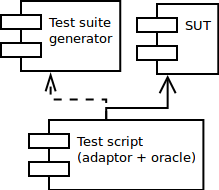
\includegraphics[scale=0.5]{img/architecture.png}
\caption{Architecture of the framework}
\label{fig:architecture}
\end{figure}

The engine of the framework is the test suite generator component (Figure \ref{fig:architecture}), that based on graph search algorithms. In the test suite generator both famous graph algorithms, the Chinese Postman and New York Street Sweeper algorithms have been implemented, so it can handle models in the form of undirected and directed graphs as well. The test suite generator realised in standalone a Python module.

The test script includes an adaptor for the SUT and a simple oracle. The test adaptor can handle models of SUTs that models are extended with an event data tag (Listing~\ref{lst:adaptorextension}).

\begin{lstlisting}[label={lst:adaptorextension}, caption=Extension of GraphML for the test adaptor,breaklines=true,basicstyle=\ttfamily\footnotesize,]
<key id="d1" for="edge" attr.name="event" attr.type="string"/>
\end{lstlisting}

The oracle of the framework simply gets the state of the SUT and compares that to the model's state.

\newpage

\subsection{Testing the framework}
\label{sub:testingtheframework}

\begin{figure}[htp]
\centering
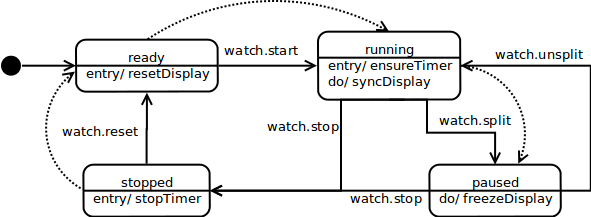
\includegraphics[scale=0.5]{img/stopwatch_eulerized.png}
\caption{Eulerized UML state diagram of the SUT}
\label{fig:stopwatch}
\end{figure}

To test the framework first a little software has been implemented, that acts like a stopwatch. The UML state diagram of the SUT can be see on Figure~\ref{fig:stopwatch}. The graph representation of this state machine does not have an Eulerian tour. The test suite generator creates a long test case that contains method calls. After the Eulerization of the graph, the Eulerian tour is going to start from the \texttt{ready} state, duplicated edges are dotted. The trace of the test execution can be see on Listing~\ref{lst:executiontrace}. In the execution trace one can see, that the methods, which are represented with a duplicated edge on the eulerized state diagram called twice (\texttt{start}, \texttt{split}, \texttt{reset} methods).

\begin{lstlisting}[label={lst:executiontrace}, caption=Test execution trace,breaklines=true,basicstyle=\ttfamily\footnotesize,]
TEST0: watch.start
Result: running
PASSED
TEST1: watch.split
Result: paused
PASSED
TEST2: watch.unsplit
Result: running
PASSED
TEST3: watch.split
Result: paused
PASSED
TEST4: watch.stop
Result: stopped
PASSED
TEST5: watch.reset
Result: ready
PASSED
TEST6: watch.start
Result: running
PASSED
TEST7: watch.stop
Result: stopped
PASSED
TEST8: watch.reset
Result: ready
PASSED
\end{lstlisting}

% subsection testingtheframework (end)

% section implementation (end)

\section{Summary and further development}
\label{sec:summary}

After investigating the model-based testing theory and its motivation we could see the advantages of this technology. The process of MBT and a possible taxonomy was described, which gave the base for a systematic tools review. Some new properties of MBT related softwares has been defined from a practical point of view. Two concrete testing framework have been presented regarding the previously described properties. Conclusion of the review can be utilised in later works.

Connection to graph theory is a cardinal part of test case generation technologies. The most usable algorithms and some variants have been discussed in that section.

Finally the work has been summarised with a creation of a complete model-based testing framework. The usability and the operation have been demonstrated with a living software.

Finding and demonstrating new technologies, algorithms can be part of the further development.

% section summary (end)

% Bibliography
\clearpage
\nocite{*}
\bibliographystyle{plain}
\bibliography{/home/chef/Egyetem/Onlab1/msc-thesis/doc/unicsovicsmilangyorgy_jzk.bib}

\end{document}
